%\documentclass[fontsize=11pt, appendixprefix=true]{scrreprt}
\documentclass[10pt]{report}
\usepackage{tocloft}
%\renewcommand{\cftpartleader}{\cftdotfill{\cftdotsep}} % for parts
%\renewcommand{\cftchapleader}{\cftdotfill{\cftdotsep}} % for chapters
\renewcommand{\cftsecleader}{\cftdotfill{\cftdotsep}} % for sections, if you really want! (It is default in report and book class (So you may not need it).

% appendixprefix: hogy odaírja, hogy "Függelék A", ne csak "A"
%\usepackage[english, magyar]{babel}                        % nyelvi csomag
\usepackage[T1]{fontenc}                                   % ékezetes betűknél is legyen automatikus elválasztás
\usepackage[utf8]{inputenc}                                % ékezetes betűk kezelése
%\usepackage{lmodern}                                       % alapértelmezett betűtípus ne legyen pixeles
%\usepackage{mathtools}                                     % képletekhez kell
\usepackage[backend=biber, sorting=anyt]{biblatex}           % bibliográfia
\usepackage{parskip}
\addbibresource{main.bib}
\usepackage{url}
\usepackage{enumitem}
\usepackage{amsmath} 
\usepackage{amssymb}
\usepackage{graphicx}                                      % képek beszúrása
%\usepackage{subcaption}
\usepackage{subfig}
\graphicspath{ {images/} }
\usepackage[export]{adjustbox}                             % ez az ITK logó pozicionálásához kell
\usepackage[margin=2.5cm, bindingoffset=1.25cm]{geometry}  % margók
\usepackage[onehalfspacing]{setspace}                      % másfeles sorköz
\usepackage[hidelinks, unicode, pdfusetitle]{hyperref}     % kattintható tartalomjegyzék és hivatkozások
\usepackage{bookmark}                                      % PDF könyvjelzők
\usepackage{csquotes}                                      % a bibliográfiában megfelelően legyenek formázva az idézőjelek
\DeclareQuoteAlias{german}{magyar}
\usepackage{blindtext} % mer mért ne?
% Kódrészletekhez ajánlom
\usepackage{listings, scrhack}
%\usepackage{sourcecodepro} % egy jó betűtípus
\lstset{captionpos=b, numberbychapter=false, basicstyle=\ttfamily, showstringspaces=false, columns=fullflexible}
% Kódrészletek magyar stílusú számozása
%\renewcommand\lstlistingname{kódrészlet}
%\makeatletter
%\renewcommand\fnum@lstlisting{\ifx\lst@@caption\@empty\else\thelstlisting.~\fi\lstlistingname}%
%\makeatother
% Nyilatkozathoz két parancs definíciója
\newcommand{\pushtobottom}{\vspace*{\fill}}
\newcommand{\signatureline}[1]{\begin{flushright}
	\vspace*{.5cm}\par\noindent\makebox[2.5in]{\hrulefill}
	\par\noindent\makebox[2.5in][c]{#1}
	\end{flushright}
}

% reference
%\usepackage[plain]{fancyref}
%\usepackage[english, nameinlink]{cleveref}

%formázás
\usepackage{hyperref}
\hypersetup{%
  colorlinks=true,% hyperlinks will be coloured
  urlcolor=blue,% hyperlink text will be green
  linkcolor=black,
  citecolor=blue
}
\usepackage{fancyhdr}
\pagestyle{fancy}
\fancyhf{}
%\fancyhead[L]{\leftmark}
\fancyhead[L]{\textsl{\leftmark}}
\fancyhead[R]{\thepage}
\renewcommand{\headrulewidth}{.001cm}

% Ezeket írd át!
\author{Csaba Botos}
\title{Bioinformatics Project}
\date{2016}
%\subject{A thesis submitted for the Council of Scientific Students’ Associations}
%\publishers{Advisor:\\PhD.\ István Z. Reguly}

\usepackage{titlesec}

% Chapter customization
\renewcommand\thesection{\arabic{section}}
\setcounter{secnumdepth}{2}

\titleformat{\chapter}[block]
  {\normalfont\Huge\bfseries}{\thechapter.}{1em}{\huge}
%\titleformat{\subsection}[block]

% For quotes
\usepackage{epigraph}
\setlength\epigraphwidth{0.7\textwidth}
\setlength\epigraphrule{0pt}

\begin{document}
%%%%%%%%%%%%%%%%%%%%%%%%%%%%%%%
%% BEVEZETÉS


\includegraphics[valign=m]{ITK_logo} \parbox[c]{\textwidth}{Pázmány Péter Catholic University\\ Faculty of Information Technology and Bionics}
\vspace*{\fill}

{\let\newpage\relax\maketitle}
\vspace*{\fill}
\begin{center}
An assignment submitted as the mid-term project of Bioinformatics.

\end{center}
\clearpage

\pagenumbering{Roman}
\chapter*{Biological overview}
\addcontentsline{toc}{chapter}{Biological overview}
The butterfly effect is somewhat present in our body too. A tiny malfunction in one area can lead to
serious diseases. Neurological diseases like Schizophrenia, Autism, Fraser syndrome and many more
rely on the wiring and connections of the brain. Moreover the mentioned diseases have been linked to
excitatory synapses. The postsynaptic density (PSD) of a synapse is a dense and active network of
proteins. Proteins in this network regulate, guide and anchor the receptors to the membrane. A large
number of PSD proteins contain the domain called PDZ. As a reminder: a domain is a building block of
a protein that carries an independent function and is usually encoded by a separate (set of) exon(s). The
PDZ domain is specialised for binding, creating the nodes of the network. Proteins containing PDZ
domains  influence the  function  of the PSD, synapses  and can  have a  clear  impact in multiple
neurological diseases
\begin{figure}
\centering
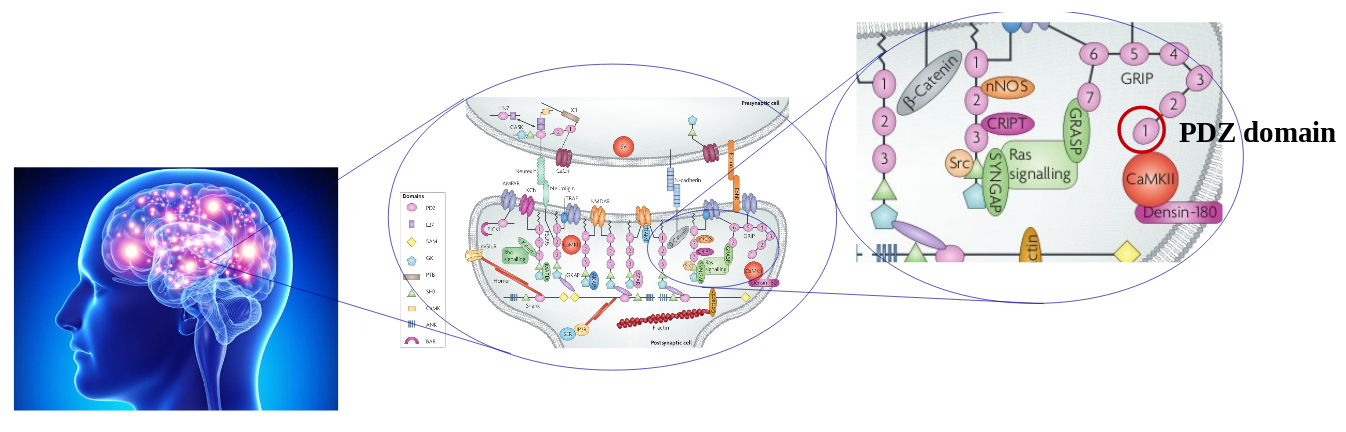
\includegraphics[width=\textwidth]{PDZ.png}
\caption{\emph{Proteins containing PDZ
domains  influence the  function  of the PSD, synapses  and can  have a  clear  impact in multiple
neurological diseases.}
Image source \href{https://wiki.itk.ppke.hu/twiki/pub/PPKE/BevBioInfo2016/bioinfo_p2016.pdf}{Assignment description}
%
}
\end{figure}
\clearpage
\chapter*{Literature}
\addcontentsline{toc}{chapter}{Literature}

A humble listing of the selected bibliography and related works, including their \emph{Abstract}. The mentioned articles and writings were used for 
the assignment.

\section{\cite{mejias2011gain} Gain-of-function glutamate receptor interacting protein 1 variants alter GluA2 recycling and surface distribution in patients with autism } Glutamate receptor interacting protein 1 (GRIP1) is a neuronal scaffolding protein that interacts directly with the C termini of glutamate receptors 2/3 (GluA2/3) via its PDZ domains 4 to 6 (PDZ4–6). We found an association (P < 0.05) of a SNP within the PDZ4-6 genomic region with autism by genotyping autistic patients (n = 480) and matched controls (n = 480). Parallel sequencing identified five rare missense variants within or near PDZ4–6 only in the autism cohort, resulting in a higher cumulative mutation load (P = 0.032). Two variants correlated with a more severe deficit in reciprocal social interaction in affected sibling pairs from proband families. These variants were associated with altered interactions with GluA2/3 and faster recycling and increased surface distribution of GluA2 in neurons, suggesting gain-of-function because GRIP1/2 deficiency showed opposite phenotypes. Grip1/2 knockout mice exhibited increased sociability and impaired prepulse inhibition. These results support a role for GRIP in social behavior and implicate GRIP1 variants in modulating autistic phenotype.

\section{\cite{feng2009organization} Organization and dynamics of PDZ-domain-related supramodules in the postsynaptic density}
As the major components of the postsynaptic density of excitatory neuronal synapses, PDZ-domain-containing scaffold proteins regulate the clustering of surface glutamate receptors, organize synaptic signalling complexes, participate in the dynamic trafficking of receptors and ion channels, and coordinate cytoskeletal dynamics. These scaffold proteins often contain multiple PDZ domains, with or without other protein-binding modules, and they usually lack intrinsic enzymatic activities. Recent biochemical and structural studies have shown that tandemly arranged PDZ domains often serve as structural and functional supramodules that could regulate the organization and dynamics of synaptic protein complexes, thus contributing to the broad range of neuronal activity.

\section{\cite{takamiya2008glutamate} The glutamate receptor-interacting protein family of GluR2-binding proteins is required for long-term synaptic depression expression in cerebellar Purkinje cells}
Glutamate receptor-interacting protein 1 (GRIP1) and GRIP2 are closely related proteins that bind GluR2-containing AMPA receptors and couple them to structural and signaling complexes in neurons. Cerebellar long-term synaptic depression (LTD) is a model system of synaptic plasticity that is expressed by persistent internalization of GluR2-containing AMPA receptors. Here, we show that genetic deletion of both GRIP1 and GRIP2 blocks LTD expression in primary cultures of mouse cerebellar neurons but that single deletion of either isoform allows LTD to occur. In GRIP1/2 double knock-out Purkinje cells, LTD can be fully rescued by a plasmid-driving expression of GRIP1 and partially rescued by a GRIP2 plasmid. These results indicate that the GRIP family comprises an essential molecular component for cerebellar LTD.
Disks large homolog 3 (DLG3) also known as neuroendocrine-DLG or synapse-associated protein 102 (SAP-102) is a protein that in humans is encoded by the DLG3 gene.[3][4] DLG3 is a member of the membrane-associated guanylate kinase (MAGUK) superfamily of proteins.
\section{\cite{dong1997grip} GRIP: a synaptic PDZ domain-containing protein that interacts with AMPA receptors}
AMPA glutamate receptors mediate the majority of rapid excitatory synaptic transmission in the central nervous system1,2 and play a role in the synaptic plasticity underlying learning and memory3,4. AMPA receptors are heteromeric complexes of four homologous subunits (GluRl–4) that differentially combine to form a variety of AMPA receptor subtypes1,2. These subunits are thought to have a large extracellular amino-terminal domain, three transmembrane domains and an intracellular carboxy-terminal domain5. AMPA receptors are localized at excitatory synapses and are not found on adjacent inhibitory synapses enriched in GABAA receptors6. The targeting of neurotransmitter receptors, such as AMPA receptors, and ion channels to synapses is essential for efficient transmission7,8. A protein motif called a PDZ domain is important in the targeting of a variety of membrane proteins to cell–cell junctions including synapses8–10. Here we identify a synaptic PDZ domain-containing protein GRIP (glutamate receptor interacting protein) that specifically interacts with the C termini of AMPA receptors. GRIP is a new member of the PDZ domain-containing protein family which has seven PDZ domains and no catalytic domain. GRIP appears to serve as an adapter protein that links AMPA receptors to other proteins and may be critical for the clustering of AMPA receptors at excitatory synapses in the brain.



\section{\cite{kim2004pdz} PDZ domain proteins of synapses}
PDZ domains are protein-interaction domains that are often found in multi-domain scaffolding proteins. PDZ-containing scaffolds assemble specific proteins into large molecular complexes at defined locations in the cell. In the postsynaptic density of neuronal excitatory synapses, PDZ proteins such as PSD-95 organize glutamate receptors and their associated signalling proteins and determine the size and strength of synapses. PDZ scaffolds also function in the dynamic trafficking of synaptic proteins by assembling cargo complexes for transport by molecular motors. As key organizers that control synaptic protein composition and structure, PDZ scaffolds are themselves highly regulated by synthesis and degradation, subcellular distribution and post-translational modification.
\clearpage
\tableofcontents
\clearpage

%% BEVEZETÉS
%%%%%%%%%%%%%%%%%%%%%%%%%%%%%%%
%% TARTALOM
\chapter{Search my protein in databases}
My choice was the \textbf{Discs Large MAGUK Scaffold Protein - DLG3}.
Where MAGUK is an abbreviation for \emph{membrane-associated guanylate kinase}.
I use Google for researching on-line, mainly found matching content on:
\begin{itemize}
\item \href{Uniprot.org}{http://www.uniprot.org/uniprot/Q62936}
\item \href{GeneCards.org}{http://www.genecards.org/cgi-bin/carddisp.pl?gene=DLG3}.
\end{itemize}

\section{What is its function?}
\begin{description}
\item[Entrez Gene Summary for DLG3 Gene]

    This gene encodes a member of the membrane-associated guanylate kinase protein family. The encoded protein may play a role in clustering of NMDA receptors at excitatory synapses. It may also negatively regulate cell proliferation through interaction with the C-terminal region of the adenomatosis polyposis coli tumor suppressor protein. Mutations in this gene have been associated with X-linked mental retardation. Alternatively spliced transcript variants have been described. [provided by RefSeq, Oct 2009]

\item[GeneCards Summary for DLG3 Gene]

DLG3 (Discs Large MAGUK Scaffold Protein 3) is a Protein Coding gene. Diseases associated with DLG3 include Non-Syndromic X-Linked Intellectual Disability and Partington Syndrome. Among its related pathways are Presynaptic function of Kainate receptors and L1CAM interactions. GO annotations related to this gene include ubiquitin protein ligase binding and protein C-terminus binding. An important paralog of this gene is DLG2.

\item[UniProtKB/Swiss-Prot for DLG3 Gene \url{DLG3_HUMAN,Q92796}]

Required for learning most likely through its role in synaptic plasticity following NMDA receptor signaling.

\item[Wikipedia]
Disks large homolog 3 (DLG3) also known as neuroendocrine-DLG or synapse-associated protein 102 (SAP-102) is a protein that in humans is encoded by the DLG3 gene.[3][4] DLG3 is a member of the membrane-associated guanylate kinase (MAGUK) superfamily of proteins.
\end{description}

\clearpage
\section{How many domains does it have and what kinds?}
According to Uniprot, DLG3 gene has \textbf{five} domains, namely the following:
\begin{description}
\item[PDZ 1] Position: 149 – 235
\item[PDZ 1] 244 – 330
\item[PDZ 1] 404 – 484	
\item[SH3] 519 – 589
\item[Guanylate kinase-like] 659 – 834	
\end{description}

\section{Which publication would you read if you started to work with this protein?}

In the first place I would like to read about \emph{Isolation of a gene (DLG3) encoding a second member of the discs-large family on chromosome}, by Smith \emph{et. al}~\cite{smith1996isolation}.
I would also consider reading Mutations in the \emph{DLG3} Gene Cause Nonsyndromic X-Linked Mental Retardation, by Tarpey \emph{et. al}~\cite{tarpey2004mutations}.

\section{Protein-protein interactions are particularly important for PDZ domains}

I have found the following literature in this topic, which are worth for further investigation:
\begin{description}
\item[PDZ domains and the organization of supramolecular complexes~\cite{sheng2001pdz}] PDZ domains are modular protein interaction domains that bind in a sequence-specific fashion to short C-terminal peptides or internal peptides that fold in a $\beta$-finger. The diversity of PDZ binding specificities can be explained by variable amino acids lining the peptide-binding groove of the PDZ domain. Abundantly represented in Caenorhabditis elegans, Drosophila melanogaster, and mammalian genomes, PDZ domains are frequently found in multiple copies or are associated with other protein-binding motifs in multidomain scaffold proteins. PDZ-containing proteins are typically involved in the assembly of supramolecular complexes that perform localized signaling functions at particular subcellular locations. Organization around a PDZ-based scaffold allows the stable localization of interacting proteins and enhances the rate and fidelity of signal transduction within the complex. Some PDZ-containing proteins are more dynamically regulated in distribution and may also be involved in the trafficking of interacting proteins within the cell.
\item[An evaluation of human protein-protein interaction data in the public domain~\cite{mathivanan2006evaluation}] Protein-protein interaction (PPI) databases have become a major resource for investigating biological networks and pathways in cells. A number of publicly available repositories for human PPIs are currently available. Each of these databases has their own unique features with a large variation in the type and depth of their annotations.
\end{description}

Especially I used the \emph{Uniprot} database to find which proteins interacts with my candidate. The result is depicted on a \emph{connection-graph} on Figure \ref{protprot}.

\begin{figure}
\centering
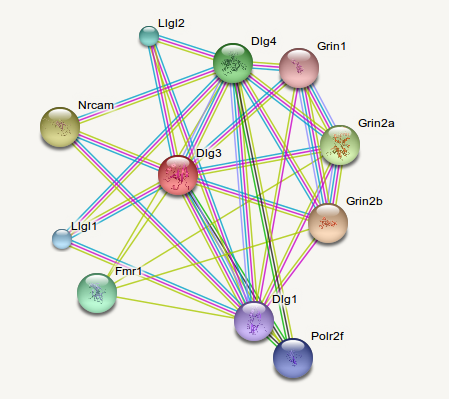
\includegraphics[width=\textwidth]{protprot.png}
\caption{\emph{Proteins containing PDZ
domains  influence the  function  of the PSD, synapses  and can  have a  clear  impact in multiple
neurological diseases.}
%
}
\label{protprot}
\end{figure}

\section{Could scientist determine a structure model for your protein yet?}

Yes, they could, a sequence model from the dabase \emph{\textsc{swiss-model}} is provided on Figure \ made with \href{http://biasmv.github.io/pv/}{PV - JavaScript Protein Viewer}

\begin{figure}
\centering
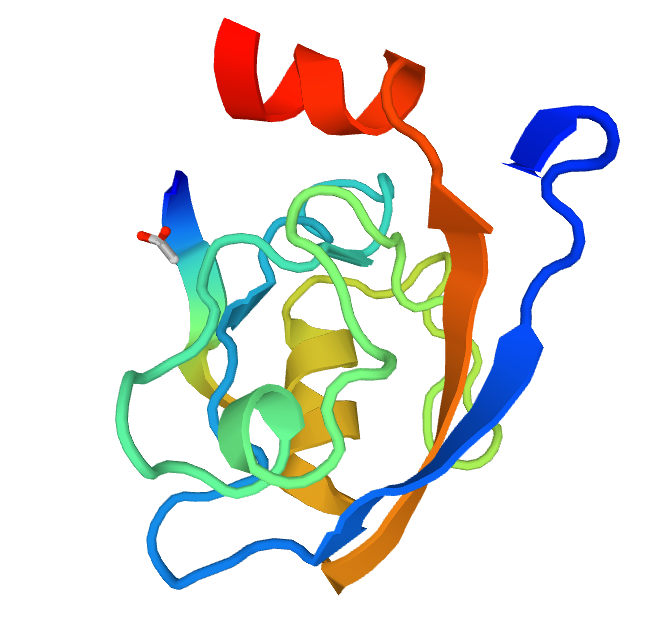
\includegraphics[width=\textwidth]{structure.png}
\caption{Sequential model of \url{DLG3_RAT}, from \href{https://modbase.compbio.ucsf.edu/modbase-cgi/model_details.cgi?queryfile=1479394245_9811&searchmode=default&displaymode=moddetail&referer=yes&snpflag=&}{\emph{\textsc{swiss-model}}}}
\label{structure}
\end{figure}

\section{Did you find anything else interesting?}
According to the results of my group mates, DLG3 is able to interact with much more protein than the others listen in the table.
It is interesting, because compared to the mentioned protein structures DLG3 has only three PDZ domains.
\clearpage
\chapter{Find and cut out domains}
I downloaded the \texttt{FASTA} from \emph{UniProt.org} with the identifier
\textbf{Q62936-1}. I sliced the three PDZ domains from the original sequence, and saved them into the corresponding \texttt{PDZ1}, \texttt{PDZ2}, \texttt{PDZ3} file available at the repository.

\section{Original File}
\lstinputlisting{files/Q62936.fasta}

\section{PDZ1}
\lstinputlisting{files/PDZ1}

\clearpage
\section{PDZ2}
\lstinputlisting{files/PDZ2}


\section{PDZ3}
\lstinputlisting{files/PDZ3}
\clearpage
\chapter{Align the domains}
For alignment, I used \href{http://www.genome.jp/tools/clustalw/}{Multiple Sequence Alignment by CLUSTALW}.

I chose the following options:
\begin{itemize}
\item Output Format: CLUSTAL
\item Gap Open Penalty: 10.0
\item Gap Extension Penalty: 0.05
\item No Weight Transition
\item Hydrophilic Residues for Proteins: \texttt{GPSNDQERK}
\item Weight Matrix: \textbf{BLOSUM} (for PROTEIN)
\end{itemize}

And the result is in \url{~/files/ex3clustal.aln}.

However, I have also found an opportunity to draw phylogenetic trees of the sequences provided. On Figure \ref{phytree1} a \emph{rooted 
phylogenetic tree with branch length} is depicted.
Probably the PDZ1 and the PDZ2 domain is replicated, because they are very close to each other, both in the DLG3 sequence and in \emph{code distance too}

\begin{figure}
\centering
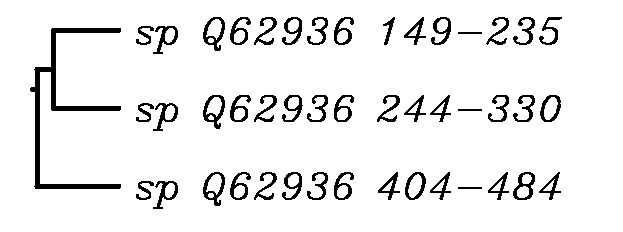
\includegraphics[width=\textwidth]{phylogenic.png}
\caption{\href{http://www.genome.jp/tools-bin/clustalwtree?treebl_upgma+1611190754597I9T9}{Source}}
\label{phytree1}
\end{figure}


\clearpage
\chapter{Compare the domains}

I used \href{http://www.bioinformatics.nl/cgi-bin/emboss/dotmatcher}{\emph{EMBOSS} \textbf{dotmatcher}}, with the following parameters:

\begin{itemize}
\item window size: 100
\item threshold: 30.00
\end{itemize}

I chose the windows size to be that large, because I wanted to see if the whole sequence could be fitted in the window, how this algorithm would recognize the domains. However, if the \texttt{threshold} was too low, then the plot became too noisy -- these considerations led to the results, which are shown on Figure \ref{dotplot}


\begin{figure}
\centering
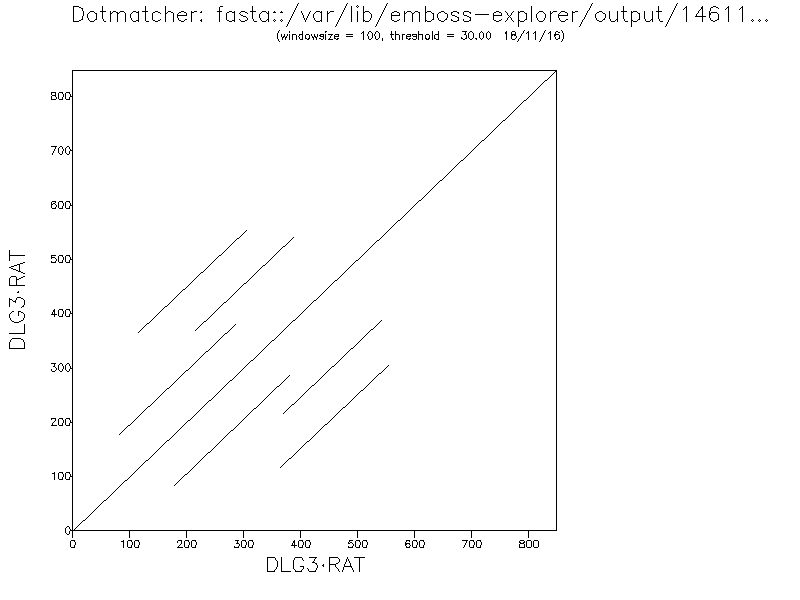
\includegraphics[width=\textwidth]{dotmatcher.png}
\caption{As seen on the picture, the \emph{three PDZ domains} are aligning to each other.
\href{http://www.bioinformatics.nl/emboss-explorer/output/146118/dotmatcher.1.png}{Source}}
\label{dotplot}
\end{figure}
\clearpage
\section{Finding similar proteins: BLAST}
\subsection{Use the NCBI BLAST for creating a database of similar proteins. Use the non-redundant protein
sequences (nr) database and restrict the search to one species.}

I visited \href{https://blast.ncbi.nlm.nih.gov/Blast.cgi?PAGE=Proteins&PROGRAM=blastp&BLAST_PROGRAMS=blastp&PAGE_TYPE=BlastSearch&BLAST_SPEC=blast2seq&DATABASE=n/a&QUERY=&SUBJECTS=}{NCBI BLAST}, and uploaded the whole sequence (\texttt{Q62936.fasta}). After I searched database \textbf{Non-redundant protein sequences (nr)} using \textbf{Blastp (protein-protein BLAST)}, I restricted the search to species \textbf{Rattus Norvegicus}. The summary of the results are shown on Figure \ref{blastsum}.

\begin{figure}
\centering
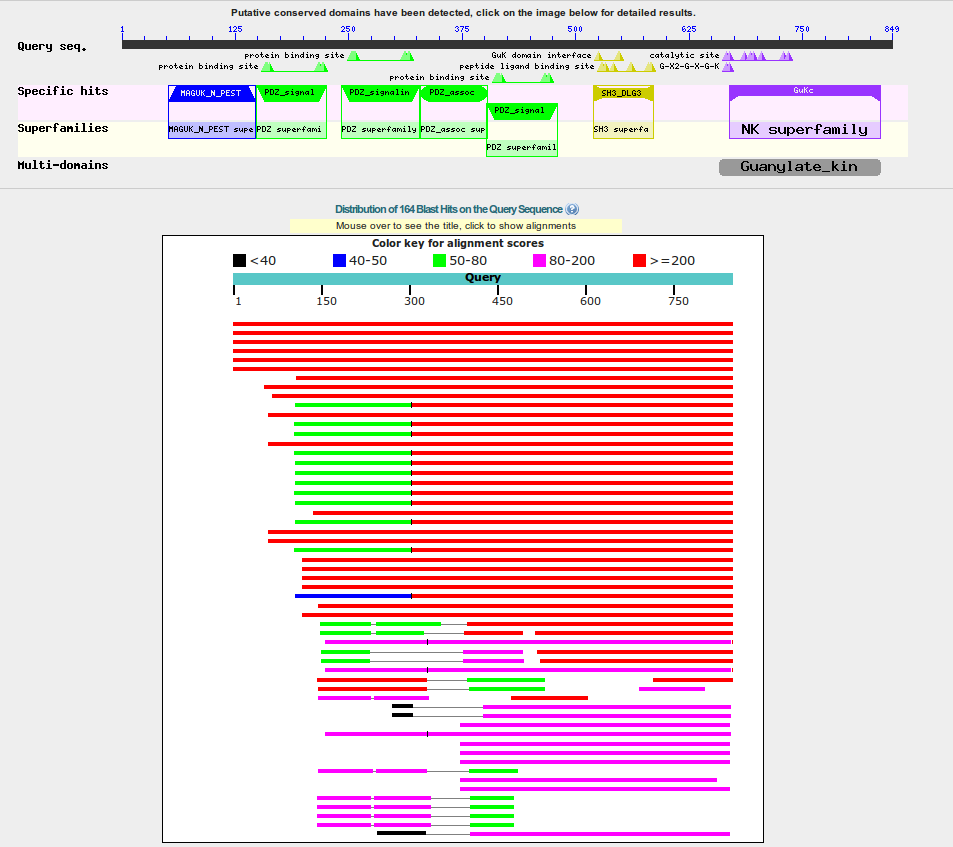
\includegraphics[width=\textwidth]{blast.png}
\caption{Result of searching database \textbf{Non-redundant protein sequences (nr)}}
\label{blastsum}
\end{figure}

As it can be seen, the search resulted in very high number of \emph{perfect} matches. This fact I would consider the hypothesis that the protein was evolutionary conserved over time, because its structure is replicated to many other similar proteins.
\paragraph{Choose 15-20 sequences from the same species BLAST hits. Shortly explain your choices.}
I chose the proteins listed in \url{~/files/ex5.fasta}, because they exhibit high level of \texttt{Query cover}, according to \href{https://blast.ncbi.nlm.nih.gov/Blast.cgi}{NCBI BLAST} and at the same time low level of actual identity.

\subsection{Create your database.}
I downloaded the proteins both in \texttt{complete} and \texttt{aligned} sequence. They can be found at: \url{~/files/ex5.fasta} and \url{~/files/ex5aligned.fasta}

\subsection{What kind of domains does blast find, are they the same as annotated in UniProtKB?}
I looked up the selected proteins on \emph{UniProtKB}, and found that the sites of match that can be seen on Figure \ref{blastsum}, are the sequences annotated in \emph{UniProtKB} as \textbf{PDZ} domains.
\clearpage
%\chapter{HMM search}
\section{Create profile HMM of PDZ domains}
I completed the \texttt{fasta} file of the initial protein PDZ domains by looking up the matching proteins from the previous example on \emph{UniProtKB},
 and downloaded their annotated PDZ domains as well, to \url{~/files/PDZ456.fasta}. After, I have merged the two file together  \url{~/files/PDZ1-6.fasta}, and multiple aligned the sequences on \url{http://www.genome.jp/tools/clustalw/}{\emph{Multiple Sequence Alignment by CLUSTALW}} with the same parameters as in Exercise 3. 
I converted the output \url{~/files/ex6-align.aln} into Stockholm format using \href{http://sequenceconversion.bugaco.com/converter/biology/sequences/index.html}{Sequence converter}, the file can be found at \url{~/files/ex6.stockholm}

For building the \textbf{HMM profile} I used the suggested \emph{hmmer} package.
The profile file can be found in \url{~/files/ex6-profile.hmm}

\section{HMM search}
First I executed \texttt{hmmer} search on the database \texttt{ex5.fasta} which I created in Exercise 5. Since I completed my PDZ profile with domains sliced from proteins of the database, the matching rate was trivially very high. 
I tested different threshold values, and saved the corresponding results in \url{ex6-mysearchE*.out} files.
With varying $E$ threshold all of the PDZ domains were found by the algorithm, (best result with $1E-40$).

Second, I used the database \emph{UniProtKB}, provided by the \href{https://www.ebi.ac.uk/Tools/hmmer/search/hmmsearch}{webserver}. Among the results I could find proteins which I have selected in my database. Compared to previous methods, this way I have found larger number of results. However the \emph{HMMer} results seems much diverse for me, while \emph{UniProt} and \emph{NCBI BLAST} listed proteins which had sequences more closer to submitted domains.

In overall, proteins with differences in their initial sequences and smaller gaps (\emph{insertion}) may originate from a common ancestor, while proteins that exhibit +99\% matching rate can be considered as a \textbf{conserved} protein.
%\clearpage
%\chapter{Phylogenetic analysis}

Because of ease of use, I chose \emph{NCBI BLAST} on \emph{UniProtKB/SwissProt} database for finding 6 mammal and a bird sequence of my protein \emph{DLG3}.
I chose the mentioned databases, because they are well supported, and validated by many researchers.

I have chosen the following sequences (6 mammal, 1 bird):
\begin{itemize}
\item \href{https://blast.ncbi.nlm.nih.gov/Blast.cgi#alnHdr_223590196}{Q12959.2}
\item \href{https://blast.ncbi.nlm.nih.gov/Blast.cgi#alnHdr_59797853}{Q811D0.1}

\item \href{https://blast.ncbi.nlm.nih.gov/Blast.cgi#alnHdr_182667930}{Q8BVD5.2}
\item \href{https://blast.ncbi.nlm.nih.gov/Blast.cgi#alnHdr_67460767}{Q5RDQ2.1}

\item \href{https://blast.ncbi.nlm.nih.gov/Blast.cgi#alnHdr_2497505}{ 	Q62696.1}
\item \href{https://blast.ncbi.nlm.nih.gov/Blast.cgi#alnHdr_71658825}{P78352.3}

\item \href{https://www.ncbi.nlm.nih.gov/protein/1708495?report=genbank&log\$=prottop&blast_rank=2&RID=33MZJTCK014}{P51527.1}
\end{itemize}

I have combined these sequences into one fasta file, \url{~/files/ex7.fasta}.
I used \href{http://www.bioinformatics.org/sms2/rev_trans.html}{\emph{Bioinformatics.org} SMS} to translate the sequences to mRNA sequences.

I multiple aligned both sequence file, using \href{http://www.genome.jp/tools-bin/clustalw}{Genome.jp CLUSTALW}, resulting in \url{~/files/ex7align.fasta}.
I also used this website's tool to generate the \emph{Rooted phylogenetic tree (UPGMA)}, with and without the branch length representing the predicted distance between species.

I also applied the suggested \textbf{R} program to compare the results.
The comparison on Figure \ref{comapre1}.
In conclusion it can be said that the original PDZ (1, 2, 3) sites are very close to each other (\texttt{Q811D0.1}, \texttt{Q62696.1}, \texttt{Q12959.2}) from phylogenetical aspect.



\begin{figure}
\centering
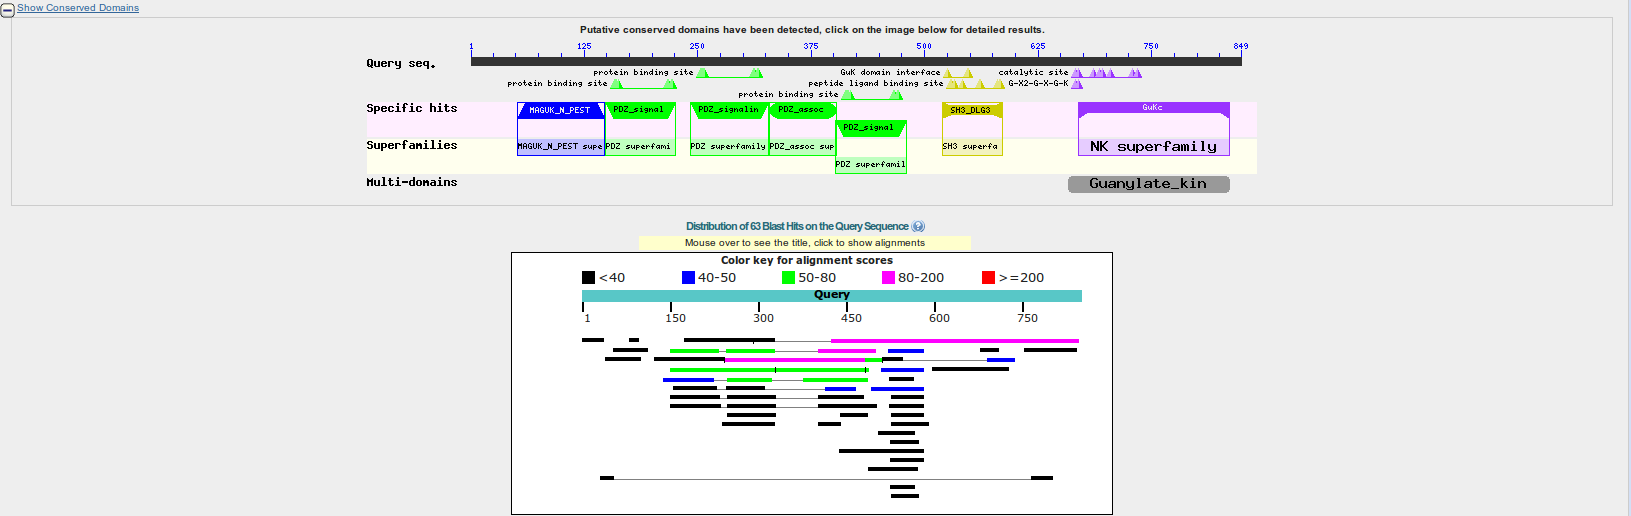
\includegraphics[width=\textwidth]{birdalign.png}
\caption{Searching for the DLG3 sequence among proteins of birds results in a poor matching, I have chosen the Sequence with the highest \texttt{Ident} value (53 \%)-}
\label{bird}
\end{figure}

\begin{figure}
\centering
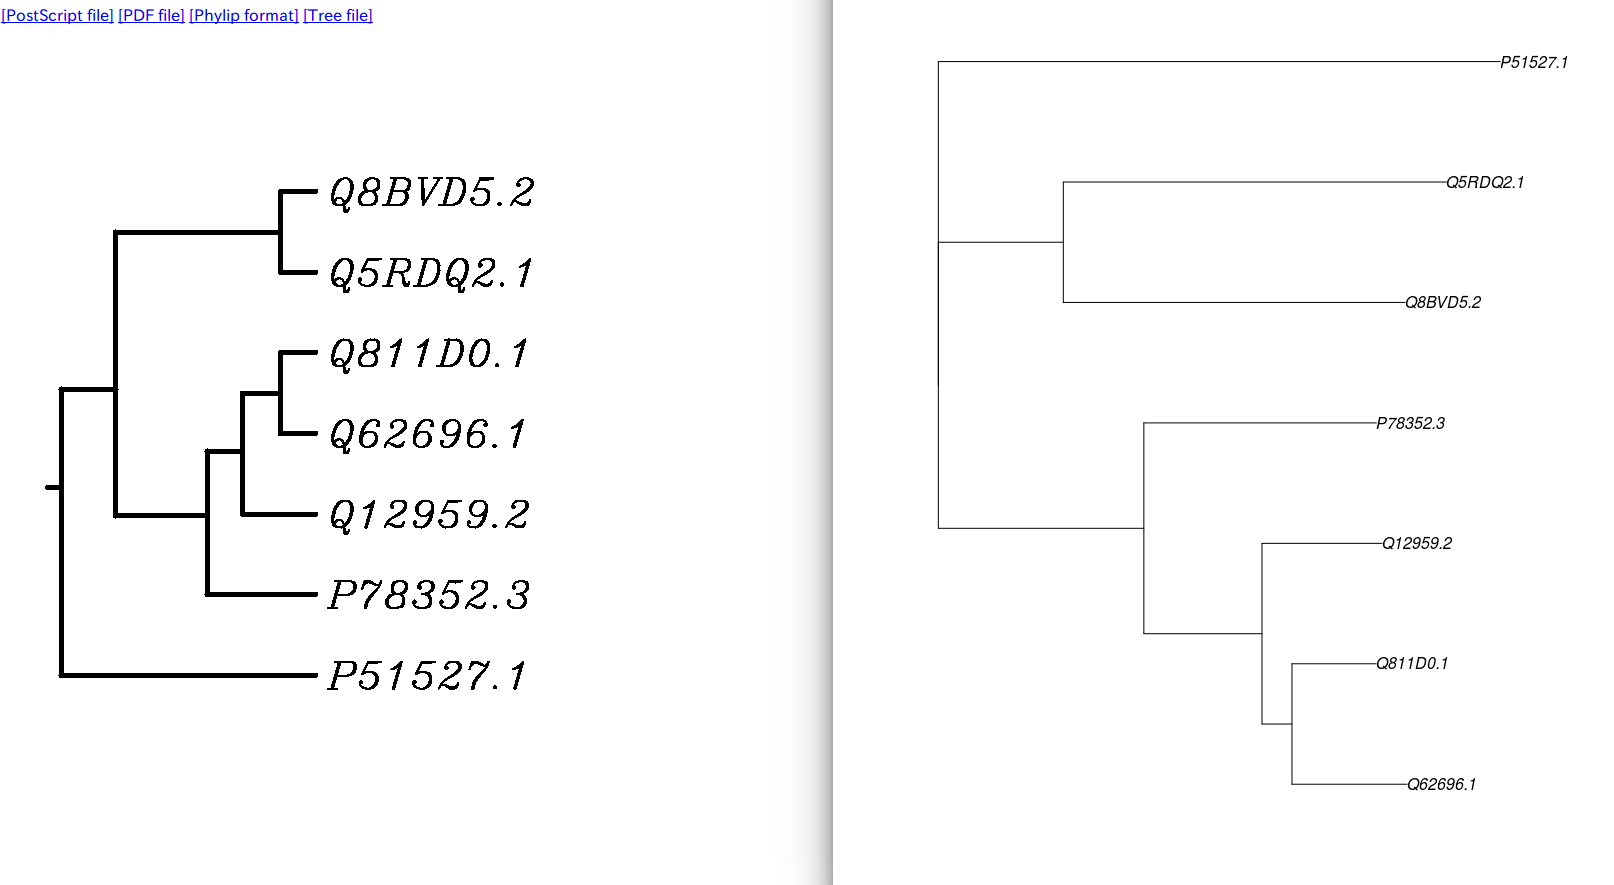
\includegraphics[width=\textwidth]{rcompare.png}
\caption{Comparing the results of \emph{R} and \emph{Genome.jp}. Except the ordering (which can be cosidered as invariant) these trees are identical. Therefore in the following I use \emph{Genome.jp} because of the user-friendly interface.}
\label{comapre1}
\end{figure}

\begin{figure}
\centering
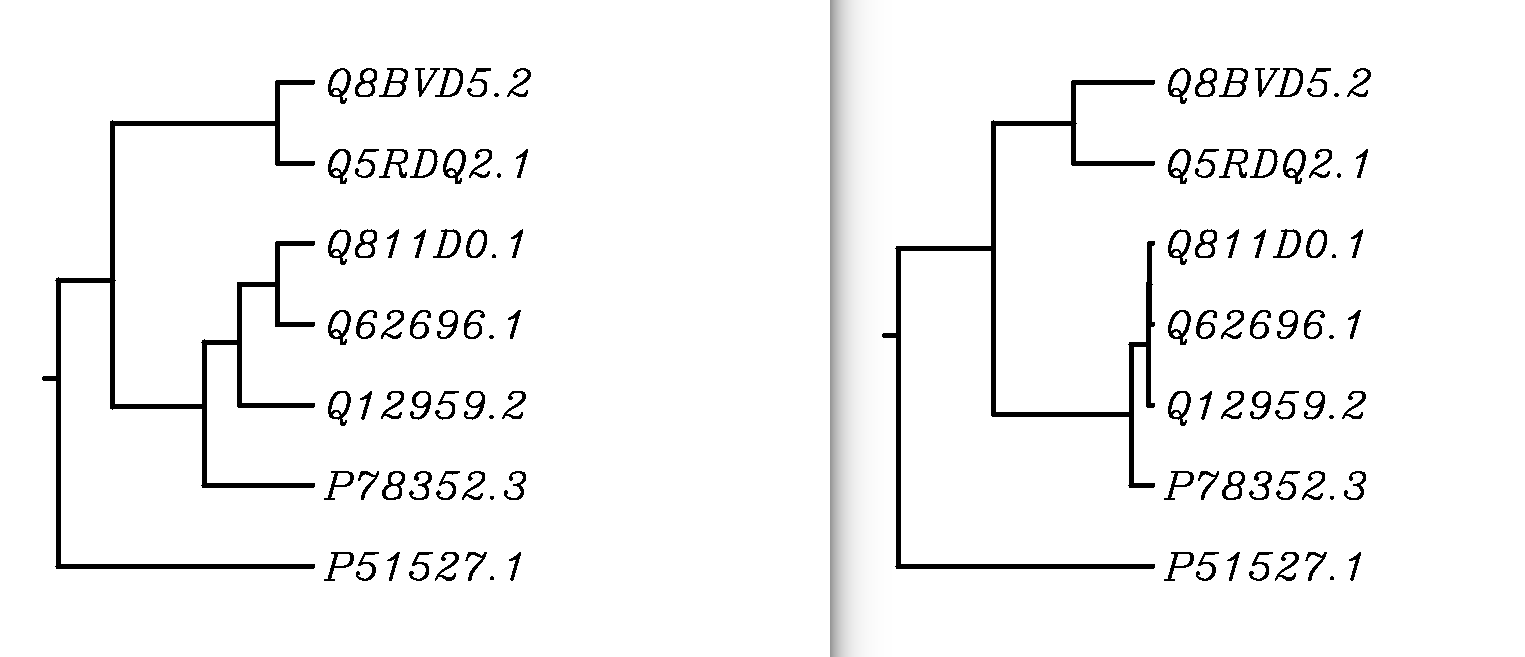
\includegraphics[width=\textwidth]{nodist-dist.png}
\caption{\emph{On the left:} Tree, showing equidistant ascension. \emph{On the right:} Tree, which branches represent the distance of the corresponding sequences. It can be seen, that the original PDZ domains fall very close to each others.}
\label{comapre2}
\end{figure}


%\clearpage
%% TARTALOM
%%%%%%%%%%%%%%%%%%%%%%%%%%%%%%%
%% BEFEJEZÉS

%\input{chapters/summary}		%
\clearpage
%\input{chapters/future}			%
\clearpage

\listoffigures
\addcontentsline{toc}{chapter}{List of Figures}
\clearpage
\printbibliography
\clearpage
%% BEFEJEZÉS
%%%%%%%%%%%%%%%%%%%%%%%%%%%%%%%
\end{document}